\section{Shape Matching}
\label{sec:shapeMatching}

Since shape detection is performed on multiple scales and shapes are extracted for small regions at a time, a heuristic is needed to determine if shapes from different nodes belong to the same structure. While on a low \textit{level-of-detail}, a wall may be contained by a single octree node, on a higher level, a node will only contain parts of the wall and multiple nodes contain primitive shapes that share this wall. This section presents a set of matching functions to determine if two shapes originate from the same geometry with a certain tolerance. Only shapes of the same type can be matching. Therefore it is not necessary to define functions to match e.g. a plane shape with a cone shape since the result will always be \verb|false|. 


\subsection{Elementary Matching Functions}
\label{sec:elementarMatchingFuns}

As the primitive shapes are represented by only a handful of parameters, it is sufficient to determine a similarity measure (called "`matching"') of these parameters. Therefore, we firstly define elementary matching functions for numbers, vectors, positions, and axes. Since matching is an approximation of equality, each matching function's result is determined by comparing a computation result to a deviation threshold $\epsilon$. If a matching function returns \verb|true| (i.e. the values don't deviate too far), the input values are considered to be matching. 

\begin{itemize}
    \item \textbf{Matching floats $f_1, f_2$}: 
        $$\frac{f_1}{f_2} \geq \epsilon, \textrm{ where } f_1 \leq f_2$$  
    \item \textbf{Matching vectors $v_1, v_2$}: 
        $$\frac{v_1}{|v_2|} \cdot \frac{v_2}{|v_2|} \geq \epsilon$$
    \item \textbf{Matching positions $p_1, p_2$}: 
        $$\sqrt{(p_1.x - p_2.x)^2 + (p_1.y - p2_y)^2 + (p1_z - p2_z)^2} \leq \epsilon$$
    \item \textbf{Matching axis $a_1, a_2$}: 
    \\
    An axis is defined by a start and end point. Let $p_{01},p_{02}$ be the start and end point of $a_1$ and $p_{11}, p_{12}$ the start and end point of $a_2$. Furthermore, let $v_1, v_2$ be the direction vectors of $a_1$ and $a_2$. The rays of the axes are denoted as $r_1 = p_{00} + sv_1$ and $r_2 = p_{10} + tv_2$. The closest distances for start and end point for each axis to the complementary ray are calculated. From those for values, the largest value $d$ is used for decision making. The matching decision is composed as follows: 
        $$\frac{v_1}{|v_2|} \cdot \frac{v_2}{|v_2|} \geq \epsilon_1 \land d \leq \epsilon_2$$
\end{itemize}


\subsection{Primitive Shape Matching Functions}
\label{sec:primitiveShapeMatchingFuns}

With the elementary matching functions defined in Section \ref{sec:elementarMatchingFuns}, it is easy to define matching functions for two primitive shapes based on the elementary matching functions:

\begin{itemize}
\item \textbf{Matching plane shapes}: 
A plane shape contains to a quad that encloses all support points. For distance computation, the plane is used, rather than the quad, since the origin of the plane shape is the plane. For each corner of each quad, the distance to the other plane is calculated. From those eight values, the largest distance $d$ is chosen. Two plane shapes are matching, if the planes' normal vectors are matching in retrospect to a threshold value $\epsilon_1$ and $d$ is smaller than or equal to a threshold value $\epsilon_2$.
\item \textbf{Matching cylinder shapes}: 
A cylinder consists of an axis and a radius. Two cylinder shapes are matching if radii and axes are matching. 
\item \textbf{Matching cone shapes}:
Cones consist of an axis, an apex, and an opening angle. Two cone shapes are matching if the axes, apexes and opening angles are matching. 
\item \textbf{Matching sphere shapes}: 
Two sphere shapes are matching if the center positions and the radii are matching. 
\item \textbf{Matching torus shapes}: 
A torus consists of a center position, an axis and a major and minor radius. Two torus shapes are matching if the center position, axes, major radii, and minor radii are matching. 
\end{itemize}

The matching result heavily depends on the chosen threshold values. Table \ref{tab:matchingThresholds} shows the $\epsilon$ values that are used for this implementation. Plane matching uses a custom heuristic that is not depicted in the table. For this heuristic, $\epsilon_2 = 0.05$ is chosen. Note that matching floats is a relative measure, whereas matching positions and axes uses world space distances as the threshold. Matching vectors uses the angle between the two vectors to calculate a matching. 

\begin{table}
\centering
\begin{tabular}{ r | r }
    Matching    & threshold values \\
    \hline
  Floats         & $\epsilon = 0.99$ \\
    Vectors     & $\epsilon = 0.95$ \\
  Positions & $\epsilon = 0.05$ \\ 
    Axis             & $\epsilon_2 = 0.05$, $\epsilon_1 = 0.95$ \\  

\end{tabular}
\caption[Different threshold values for parameter matching]
{The different threshold values for parameter matching.}
\label{tab:matchingThresholds}
\end{table}


\section{Shape Clustering}
\label{sec:shapeClustering}

With the user interaction in mind, it is not sufficient to interact with a single shape only. To determine the global extent of a primitive shape, more information is needed. Section \ref{sec:primitiveShapeMatchingFuns} describes a set of heuristics to determine if two primitive shapes originate from the same geometry. These heuristics are used in this section in order to create larger representations of a primitive shape. 
\textit{Shape Clustering} aims to find matching primitive shapes for a base shape and build a larger coherent cluster of primitive shapes over multiple level-of-details [// achtung: level of detail richtig zu verwenden. es gehört so: ein level of detail, mehrere levels of detail oder detail levels. bitte bessere das überall aus]. The types of primitive shapes can be categorized as finite and infinite shapes. Spheres and tori are finite objects per definition, thus it is sufficient enough to find a set of matching primitive shapes to create a cluster. For infinite shapes, such as planes, cones, and cylinder, additional computations are needed in order to create a coherent shape cluster. Figure \ref{fig:cuboids} shows the case of two cuboids, whose front face share a plane. By only using the matching functions to create a cluster, both front faces are packed into the cluster, even tough there is a visible gap between them.

\begin{figure}
    \centering
    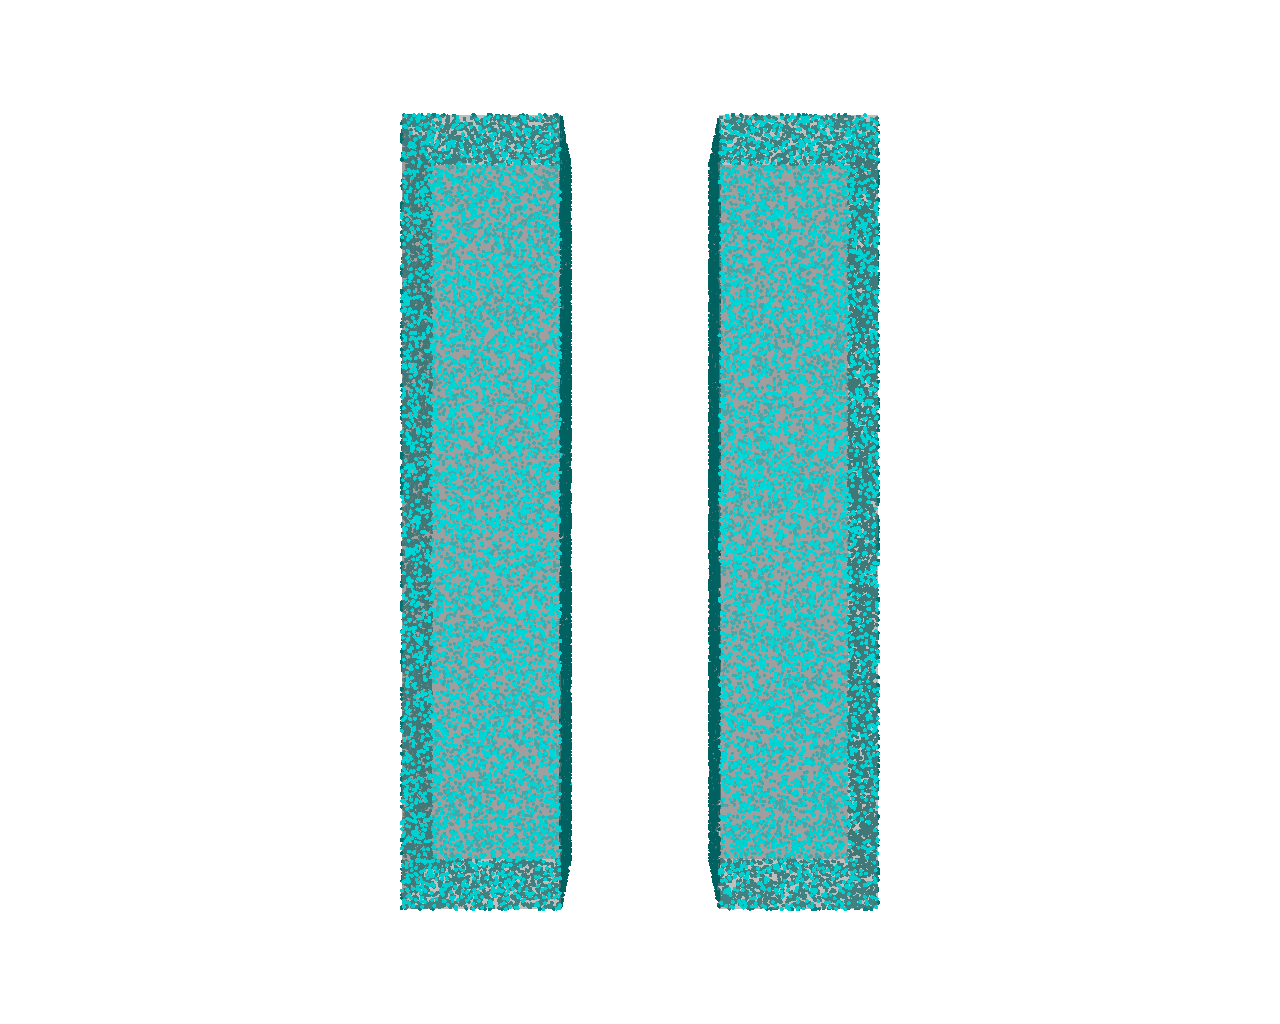
\includegraphics[width=0.8\textwidth]{Shape_Detection/cuboids.png}
    \caption[Point cloud consisting of two cuboids.]
		{A generic point cloud of two cuboids. The detected planes are rendered in grey.}
    \label{fig:cuboids}
\end{figure}

Section \ref{sec:matchingSetBuilding} describes the procedure of finding matching shapes in the octree. For infinite shapes, an additional step is performed using a region-growing approach described in Section \ref{sec:regionGrowing}. 


\subsection{Building a set of matching primitive shapes}
\label{sec:matchingSetBuilding}

In order to find matching shapes, the octree is searched for primitive shapes that match the base shape. Only octree nodes are searched that are currently rendered, such that the cluster only consists of shapes that are present in the scene. Already, the cluster consists of shapes that share the same geometry as origin. For sphere and torus shapes, this step is sufficient enough to create a valid cluster, since both shapes are finite. 


\subsection{Graph-based Region Growing}
\label{sec:regionGrowing}

A cluster of shapes can be seen as an $\epsilon$-connected component from a larger graph. A complete graph is created using all matching shapes as vertices. In a complete graph, an edge exists for any pair of vertices. The weight of an edge is determined by a custom distance function for each primitive shape:

\begin{itemize}
    \item \textbf{Plane Shape}:         As a plane shape is bounded by a quad, the distance between two plane shapes is computed as the shortest distance between the two bounding quads.
    \item \textbf{Cylinder Shape}:    The shortest distance between two cylinder shapes is determined by the shortest distance of all pairs of start/end points of both cylinders. 
  \item \textbf{Cone Shape}:            The shortest distance between two cone shapes is determined by the shortest distance of all pairs of start/end points from both cones. 
\end{itemize}


A cluster is created by growing a region in a graph, adding only vertices that connect to the current region via an edge, whose weight is smaller than $\epsilon$. This creates a cluster of shapes, ensuring that the distance to the closest neighboring shape is at maximum $\epsilon$. 
\\
\begin{figure}
    \centering
    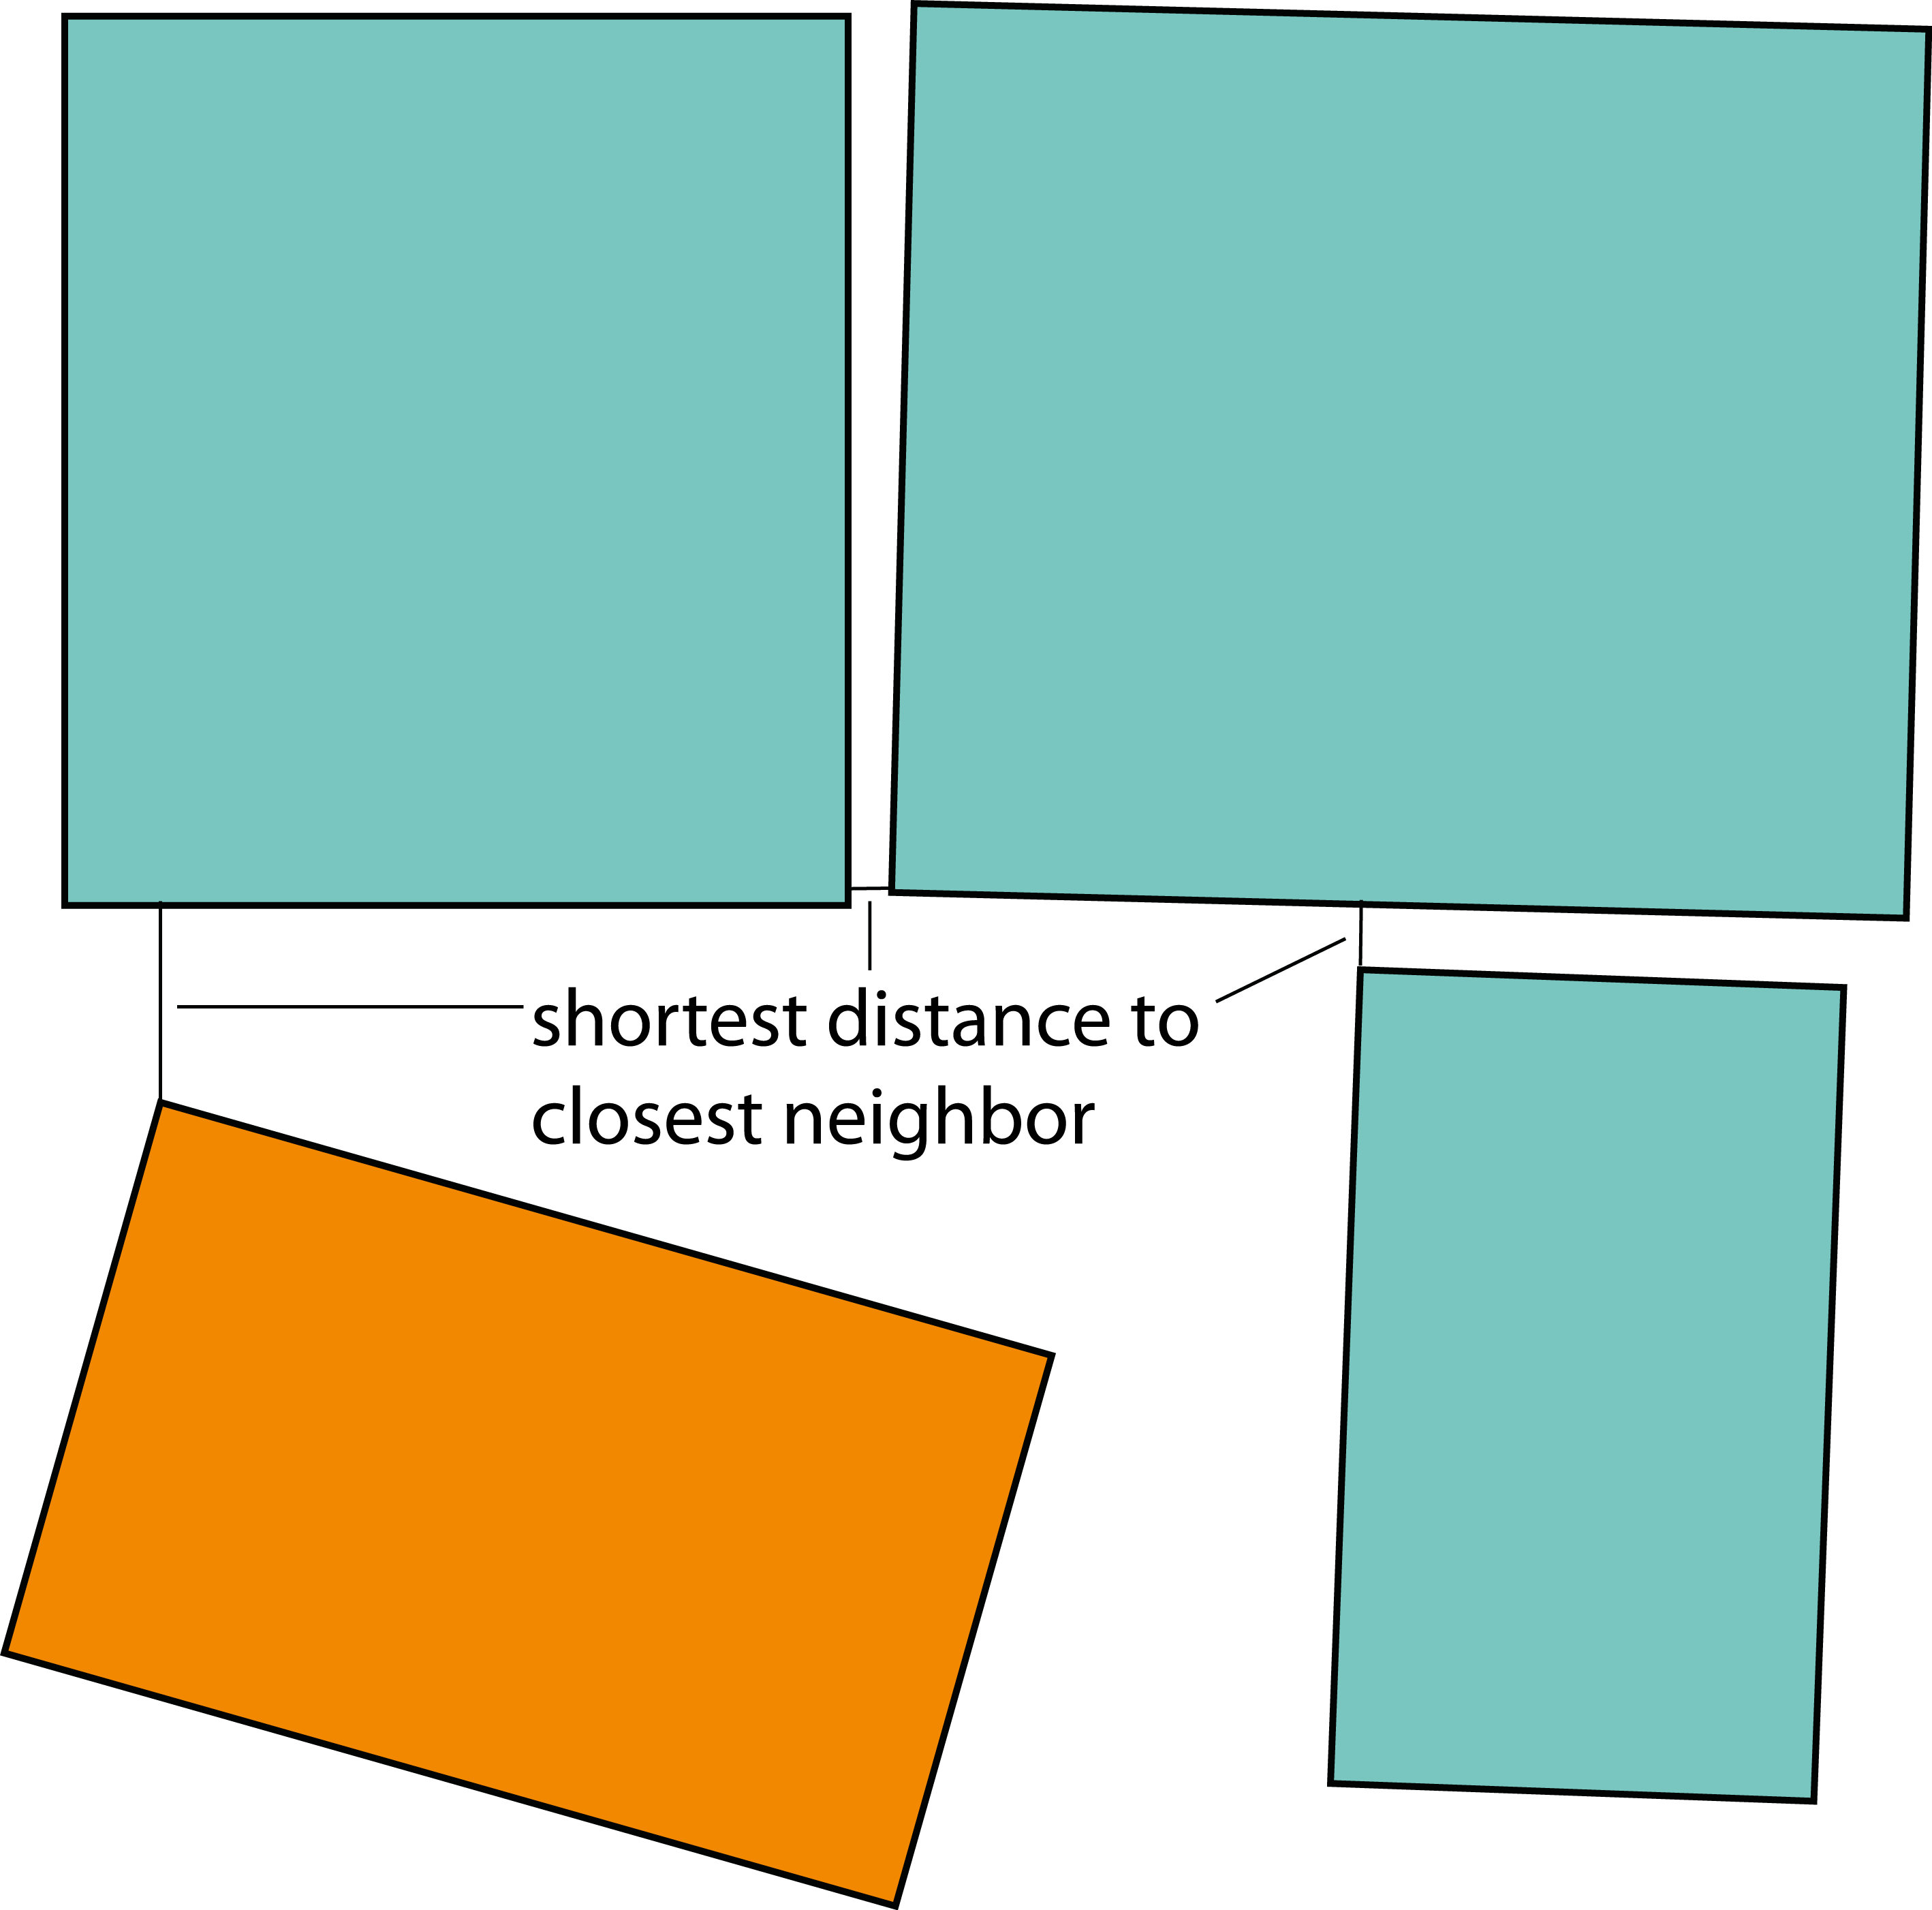
\includegraphics[width=0.5\textwidth]{Shape_Detection/regionGrowingPlanes.png}
    \caption[Exemplary $\epsilon$-connected plane cluster]
		{A cluster of plane shapes created by computing the $\epsilon$-connected component. Planes that belong to the cluster are colored in turquoise.}
    \label{fig:regionGrowingPlanes}
\end{figure}

Figure \ref{fig:regionGrowingPlanes} shows an exemplary illustration on region growing for plane shapes. The distance between two plane shapes is measured as the closest distance between the two bounding quads. 

\begin{figure}
\centering
\subcaptionbox{ \label{fig:regionGrowingCylinder}}{%
  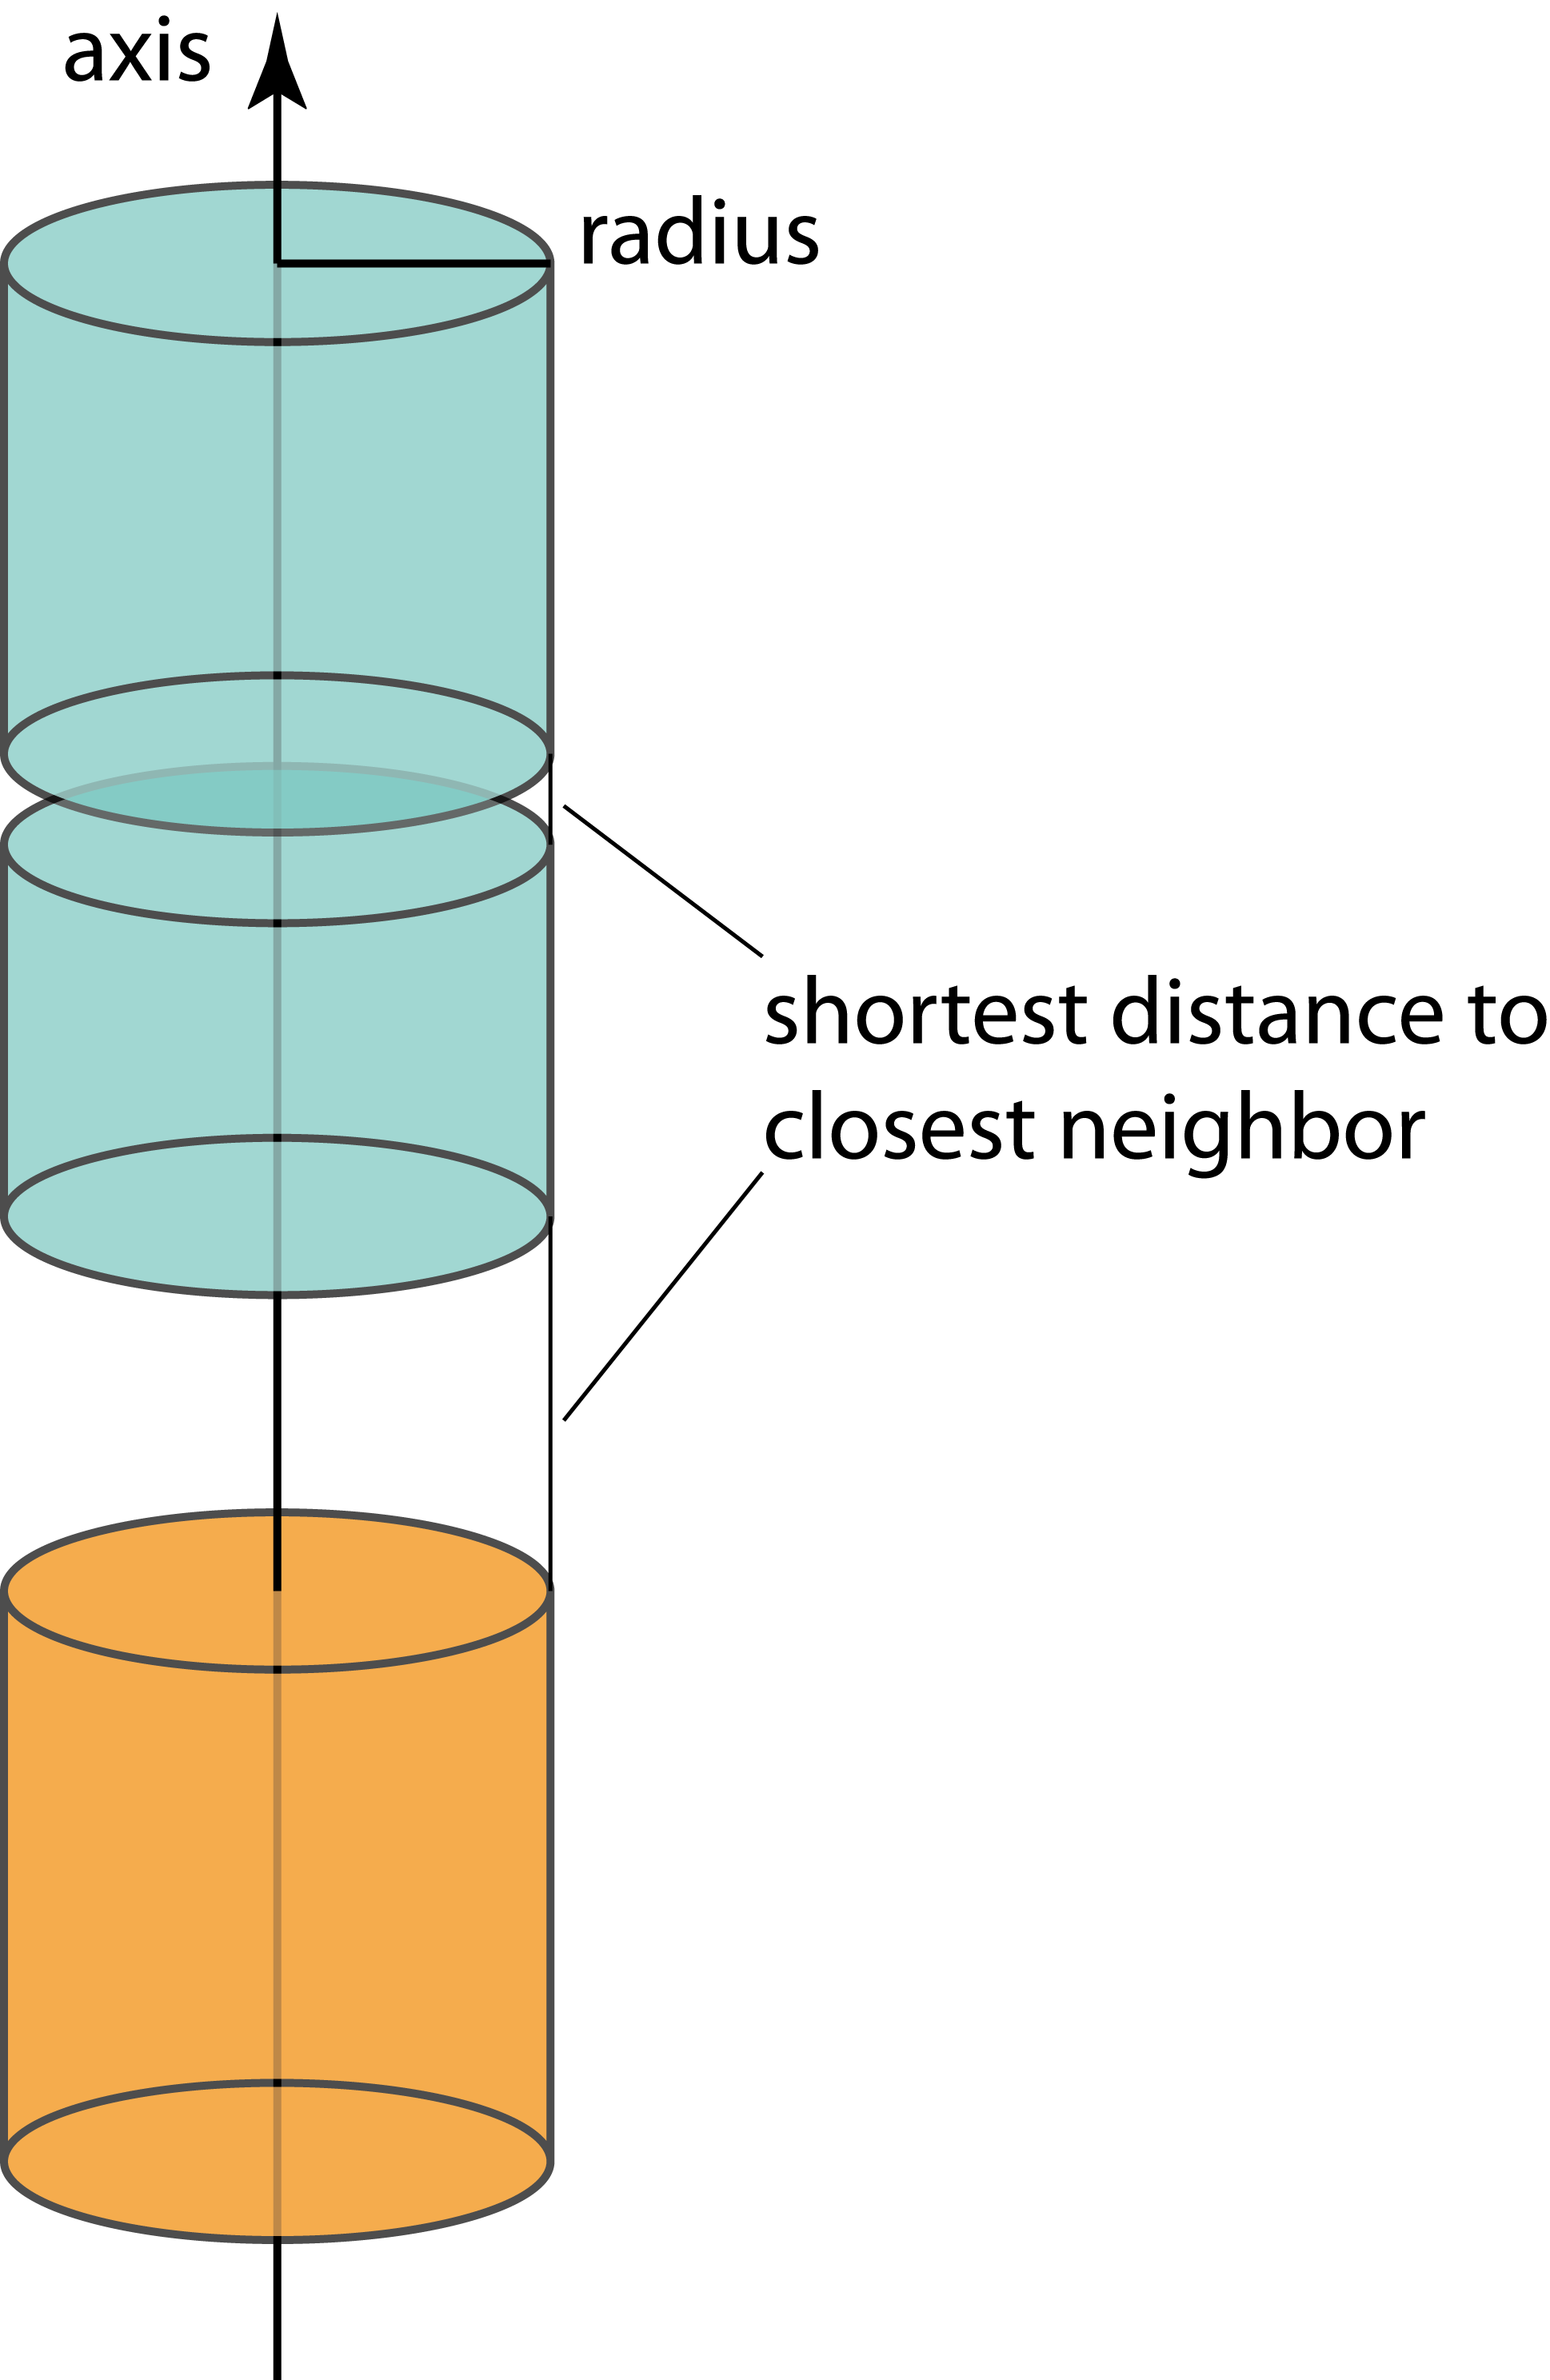
\includegraphics[width=0.3\textwidth]{Shape_Detection/regionGrowingCylinder.png}%7
  }
\subcaptionbox{ \label{fig:regionGrowingCone}}{%
  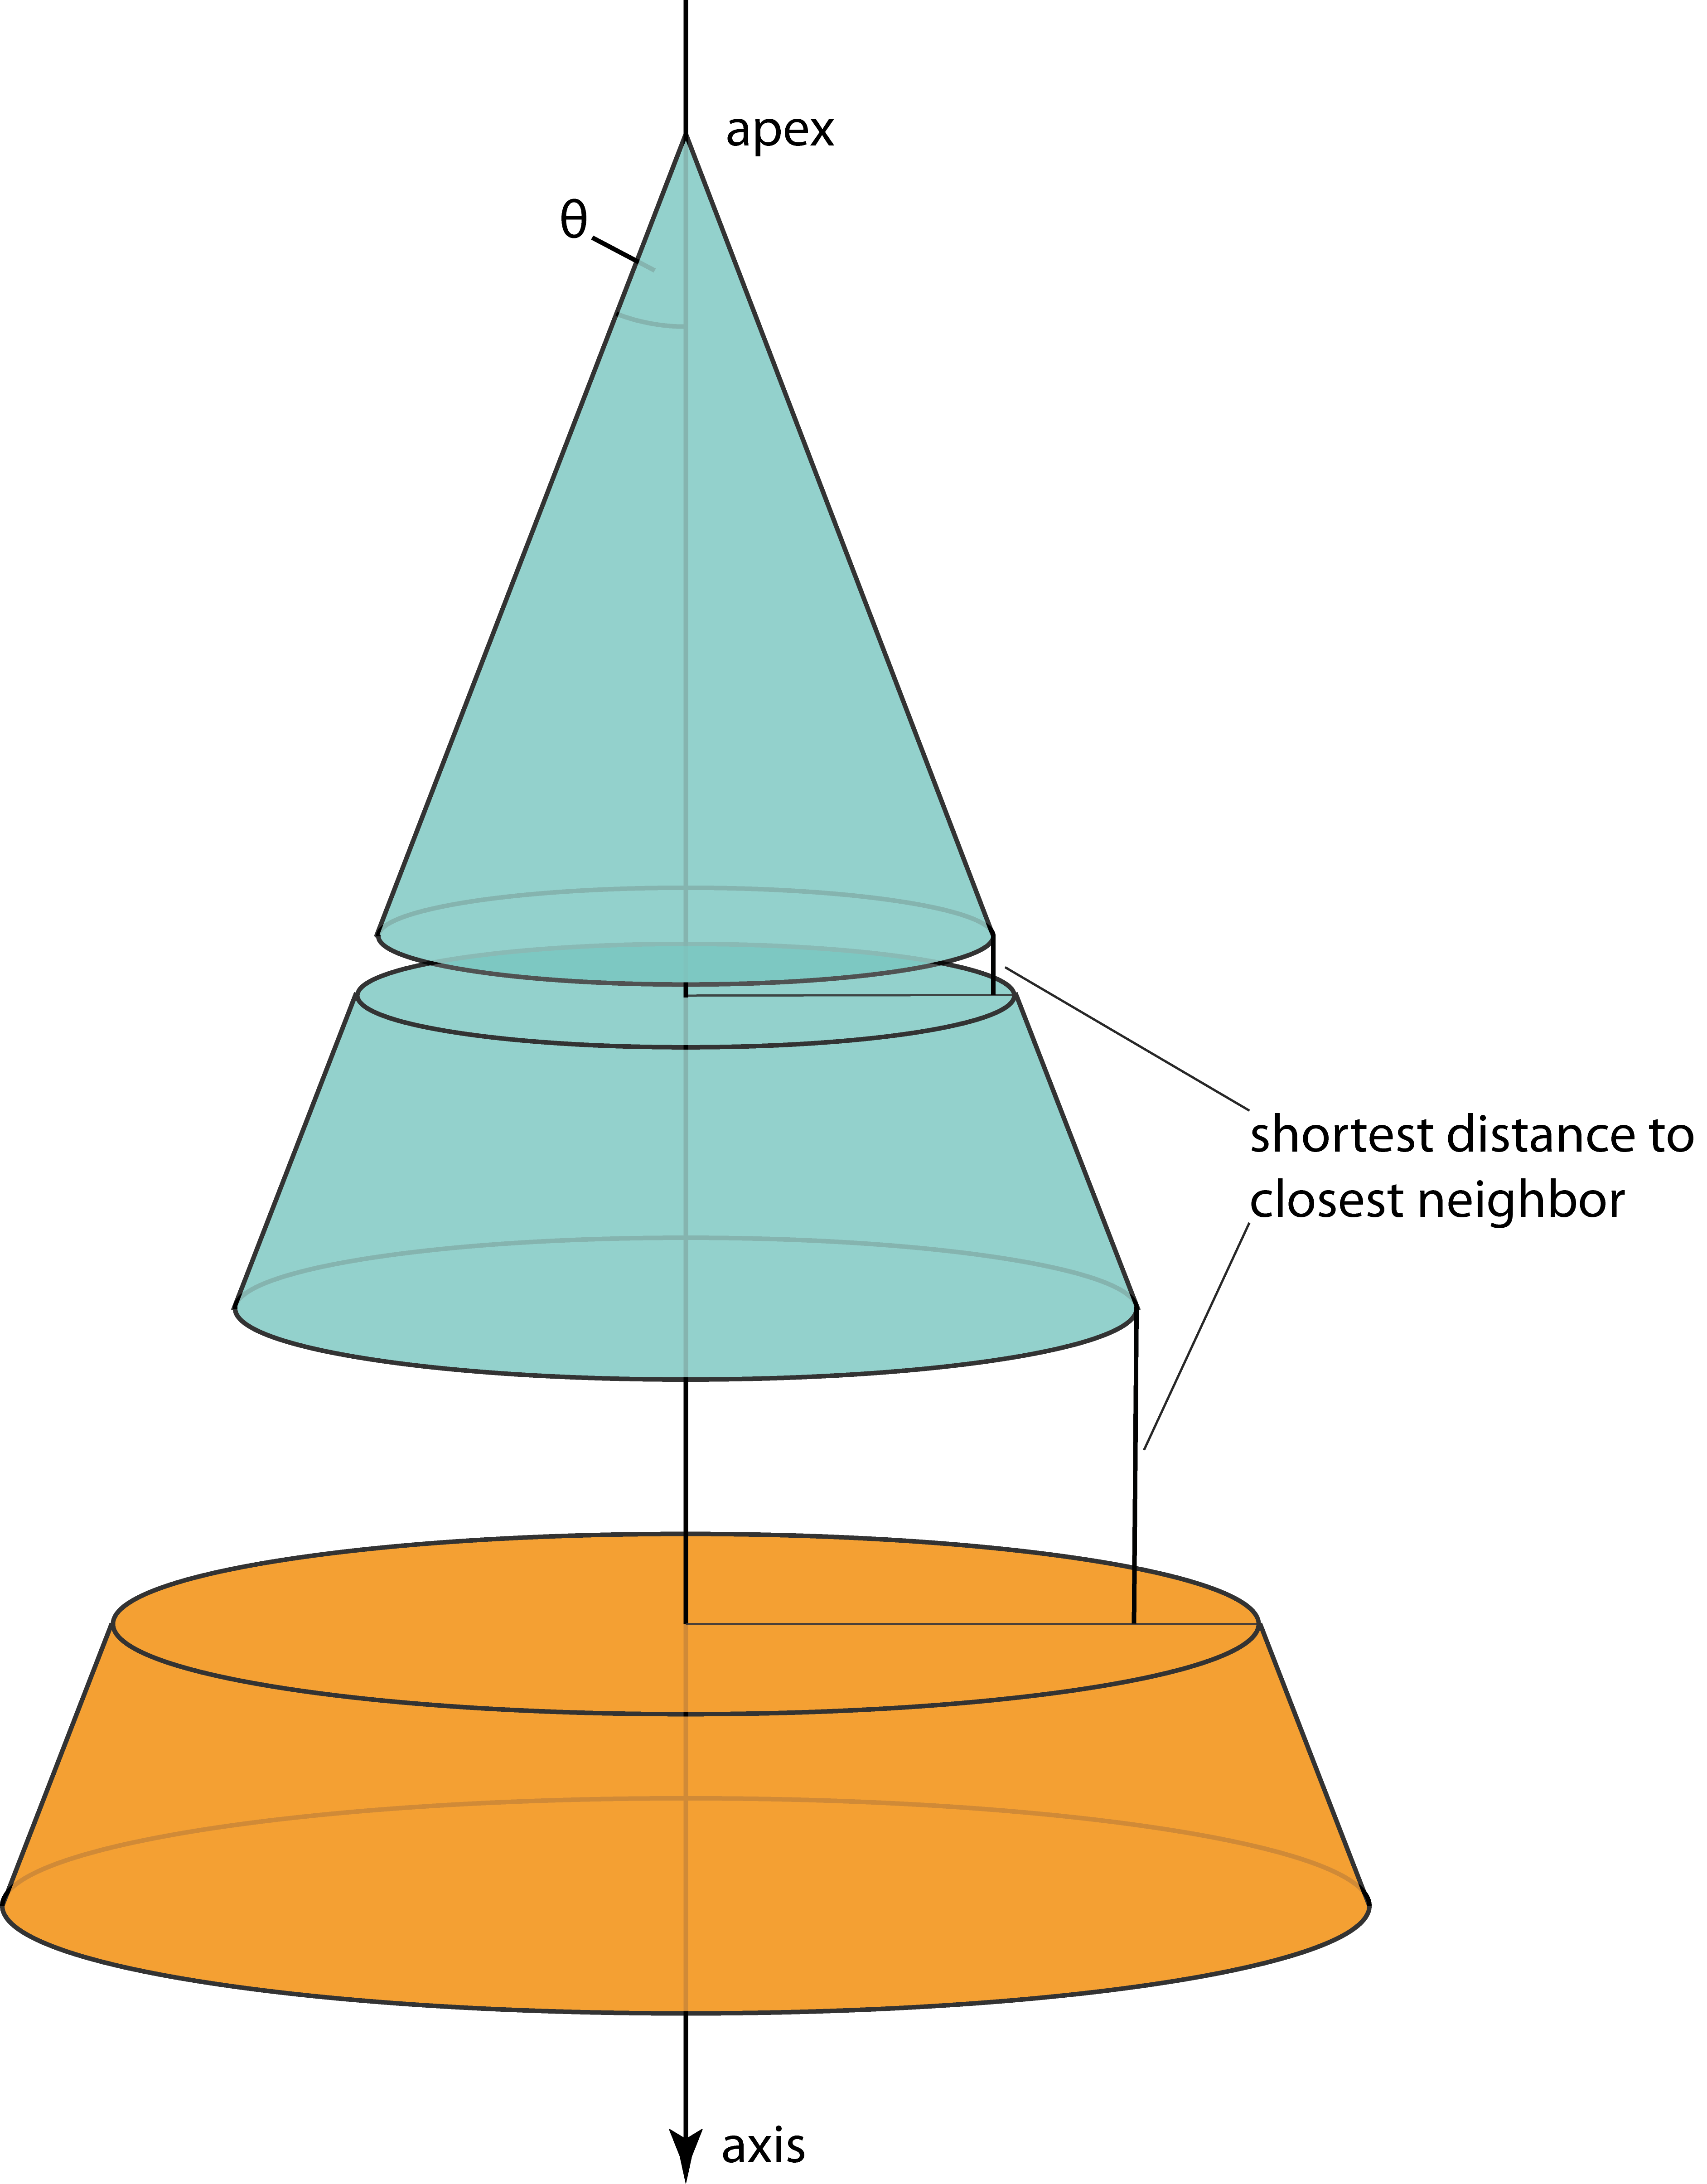
\includegraphics[width=0.5\textwidth]{Shape_Detection/regionGrowingCone.png}%
  }
    \caption[Exemplary cylinder and clone cluster]
		{This figure shows a cylinder cluster and a cone cluster build from matching shapes. Shapes that belong to the cluster are colored in turquoise.}
    \label{fig:regionGrowingConeCylinder}
\end{figure}

Figure \ref{fig:regionGrowingConeCylinder} showcases region growing for both, cylinder shapes and cone shapes. The matching heuristic already confirms that the shapes lie on the same axis and share a similar radius. Therefore, instead of a three-dimensional world distance, a one-dimensional distance between two points is sufficient to build a shape cluster. 
\\
\\
The region growing component of the clustering heavily depends on the $\epsilon$ distance threshold. A proper distance threshold that mirrors the region's topology well is the density of an octree node as described in Section \ref{sec:shapeDetectionParameterSelection}. For this task, we chose the density of the node of the base shape, more specific: $\epsilon = density \cdot 2.0$.